\documentclass[17pt, a1paper, portrait, margin=17mm, innermargin=15mm,
               blockverticalspace=3mm, colspace=7mm, subcolspace=4mm]{tikzposter}

\usepackage[T1]{fontenc}
\usepackage[utf8]{inputenc}
\usepackage{lmodern}
\usepackage{amsmath,amssymb,amsfonts}
\usepackage{bbm}
\usepackage{graphicx}
\usepackage{booktabs}
\usepackage{multirow}
\usepackage{xcolor}
\usepackage{microtype}

\graphicspath{{../slides/}{./}}
\usetikzlibrary{arrows.meta, positioning}

\title{Image Plagiarism Detection with Equivariant Encoders}
\author{Denis Gudkov \quad\textbullet\quad Daniil Dorin}
\institute{Intelligent Systems, MIPT \\[2pt]
\texttt{gudkov.da@phystech.edu} \quad\textbullet\quad \texttt{dorin.dd@phystech.edu}}

% ------------------------- Visual theme -------------------------
\definecolor{nipsblue}{HTML}{1F3A5F}
\definecolor{nipsaccent}{HTML}{C0392B}
\definecolor{nipslight}{HTML}{EAF0F6}
\definecolor{nipsgray}{HTML}{4A4A4A}

\definecolorstyle{NeurIPSPoster}{
  \definecolor{colorOne}{named}{nipsblue}
  \definecolor{colorTwo}{named}{nipslight}
  \definecolor{colorThree}{named}{nipsaccent}
}{
  \colorlet{backgroundcolor}{white}
  \colorlet{framecolor}{nipsblue}
  \colorlet{titlefgcolor}{white}
  \colorlet{titlebgcolor}{nipsblue}
  \colorlet{blocktitlebgcolor}{nipsblue}
  \colorlet{blocktitlefgcolor}{white}
  \colorlet{blockbodybgcolor}{white}
  \colorlet{blockbodyfgcolor}{nipsgray}
  \colorlet{innerblocktitlebgcolor}{nipslight}
  \colorlet{innerblocktitlefgcolor}{nipsblue}
  \colorlet{innerblockbodybgcolor}{white}
  \colorlet{innerblockbodyfgcolor}{nipsgray}
  \colorlet{notefgcolor}{nipsblue}
  \colorlet{notebgcolor}{nipslight}
  \colorlet{noteframecolor}{nipsblue}
}

\usetheme{Simple}
\usecolorstyle{NeurIPSPoster}
\usetitlestyle{Empty}
\usebackgroundstyle{Plain}

% Slim block style: shorter title bar, no frame, lighter weight title.
\defineblockstyle{Slim}{
    titlewidthscale=1, bodywidthscale=1, titleleft,
    titleoffsetx=0pt, titleoffsety=0pt,
    bodyoffsetx=0pt, bodyoffsety=8mm,
    bodyverticalshift=5mm, roundedcorners=3, linewidth=0pt,
    titleinnersep=2.5mm, bodyinnersep=5mm
}{
    \draw[draw=none, fill=blockbodybgcolor,
        rounded corners=\blockroundedcorners] (blockbody.south west)
        rectangle (blockbody.north east);
    \ifBlockHasTitle
    \draw[draw=none, fill=blocktitlebgcolor,
        rounded corners=\blockroundedcorners] (blocktitle.south west)
        rectangle (blocktitle.north east);
    \fi
}
\useblockstyle{Slim}

% Make block titles smaller and not bold-heavy.
\makeatletter
\let\origblock\block
\renewcommand{\block}[2]{\origblock{\fontsize{22pt}{24pt}\selectfont\mdseries #1}{#2}}
\makeatother

% Title rendered in an explicit paperwidth-bounded box so it never overflows.
\settitle{
  \centering
  \begin{minipage}{0.86\paperwidth}
    \centering
    {\color{nipsblue}\rule{\linewidth}{1.5pt}}\\[6pt]
    {\color{nipsblue}\bfseries\fontsize{52pt}{60pt}\selectfont \@title\par}\vspace{8pt}
    {\color{nipsgray}\fontsize{28pt}{34pt}\selectfont \@author\par}\vspace{4pt}
    {\color{nipsgray}\fontsize{22pt}{28pt}\selectfont \@institute\par}\vspace{6pt}
    {\color{nipsblue}\rule{\linewidth}{1.5pt}}
  \end{minipage}
}

\begin{document}
\maketitle

% ===================== Row 1: Abstract =====================
\block{Why Equivariant Encoders}{
A pirated image is rarely a pixel-perfect copy: rotations, reflections, crops, and JPEG re-compression are routine, and a detector should map all of them to the same point in feature space. Should this invariance be built into the encoder of a siamese plagiarism detector, or approximated through geometric augmentation at training time? To answer this question, we test $D_4$-, and $SE(2)$-equivariant encoders in the task of detecting image plagiarism. Here $D_4$ is the group of symmetries of the square and $SE(2)$ is the group of continuous roto-translations of the plane.

}

% ===================== Row 2: Pipeline | Loss =====================
\begin{columns}
\column{0.58}
\block{Siamese Network with a $G$-invariant Encoder}{
\begin{center}
  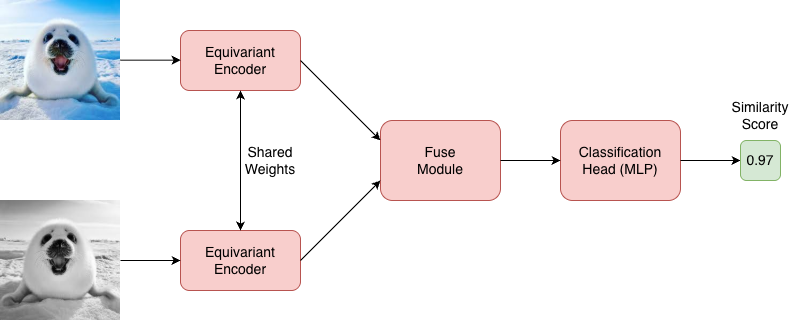
\includegraphics[width=\linewidth]{siamese-equivariant-pipeline.png}
\end{center}
\vspace{12pt}
The detector is $f_\theta(x_1,x_2)=\sigma\bigl(h_\psi(\phi_\theta(x_1),\phi_\theta(x_2))\bigr)$. The shared encoder $\phi_\theta:\mathcal{X}\!\to\!\mathbb{R}^d$ is chosen $G$-invariant, so $\phi_\theta(g\!\cdot\!x)=\phi_\theta(x)$ for all $g\!\in\!G$: geometric variants of one image collapse to a single point. The symmetric fusion head builds $\delta=|z_1-z_2|$, $p=z_1\!\odot\!z_2$, sets $v=[\delta;p]\!\in\!\mathbb{R}^{2d}$, and returns the plagiarism logit through a two-layer MLP.
}

\column{0.42}
\block{Equivariance}{
\centering
\begin{tikzpicture}[every node/.style={font=\small}, >={Stealth[length=3mm]}, thick]
  \node[inner sep=1pt] (I)   at (0,0)   {
\includegraphics[width=4.2cm]{image.png}};
  \node[inner sep=1pt] (RI)  at (8.5,0) {
\includegraphics[width=4.2cm,angle=90]{image.png}};
  \node[inner sep=1pt] (fI)  at (0,-7)  {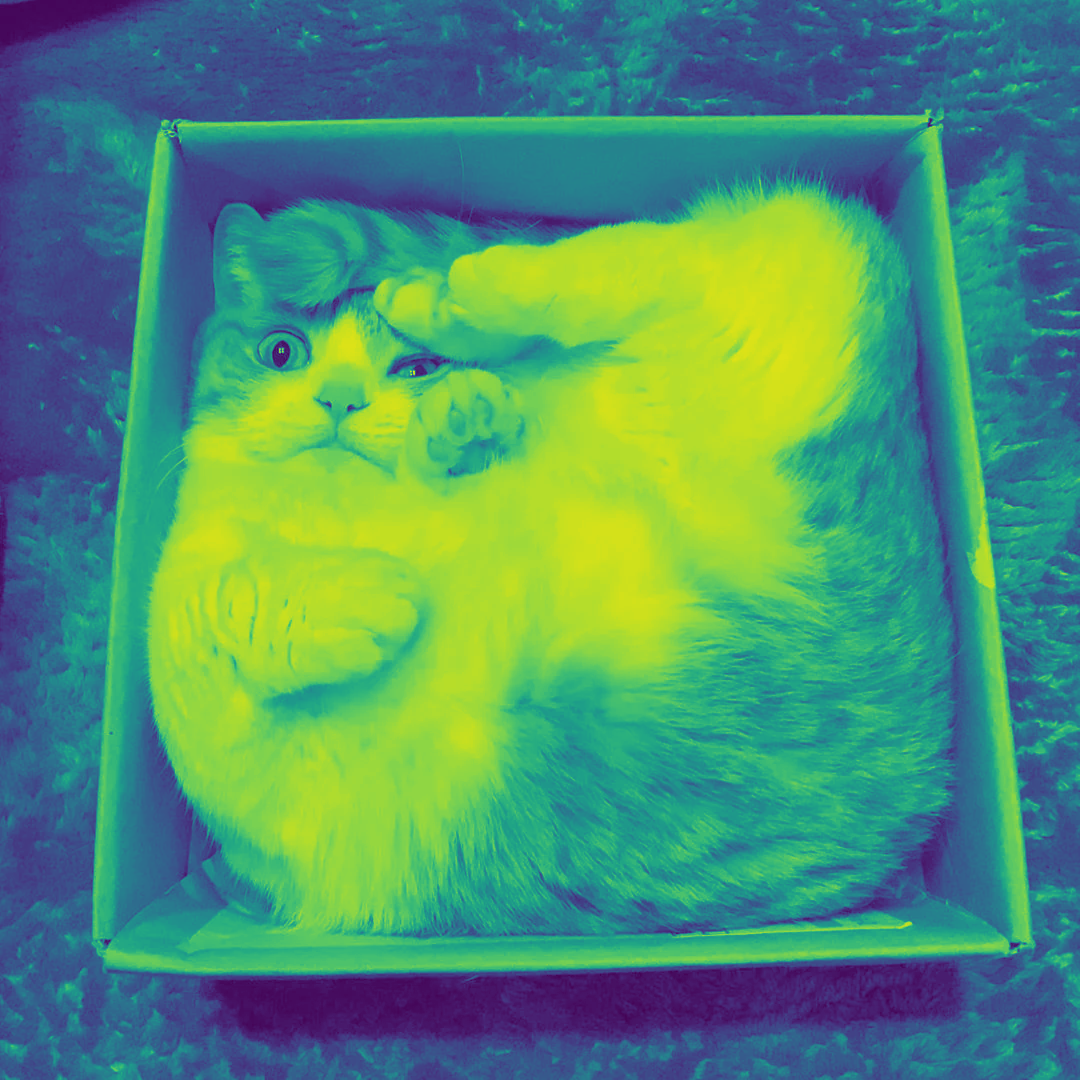
\includegraphics[width=4.2cm]{image_feat.png}};
  \node[inner sep=1pt] (RfI) at (8.5,-7){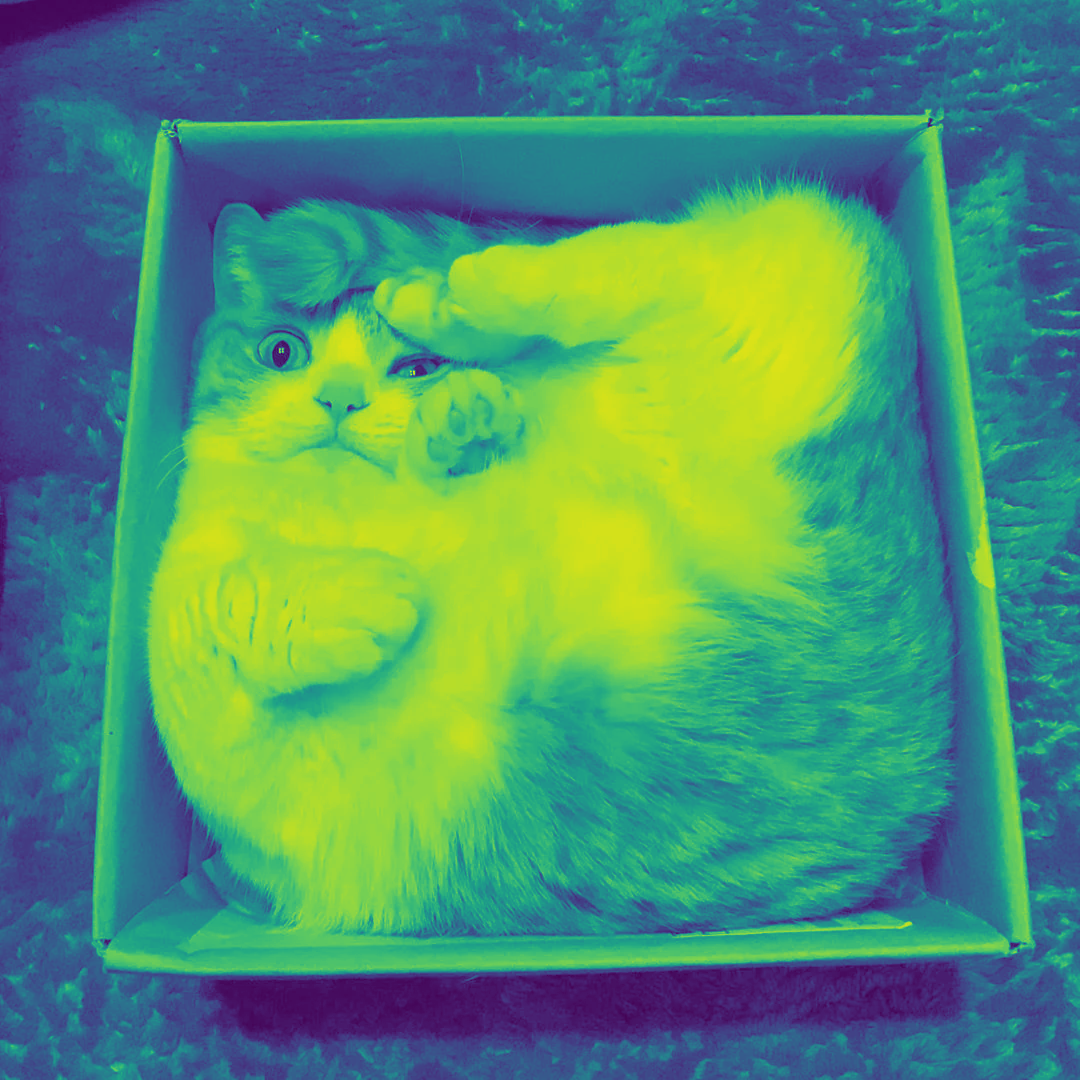
\includegraphics[width=4.2cm,angle=90]{image_feat.png}};

  \node[above=2pt of I]   {\normalsize $x$};
  \node[above=2pt of RI]  {\normalsize $g\!\cdot\!x$};
  \node[below=2pt of fI]  {\normalsize $\phi_\theta(x)$};
  \node[below=2pt of RfI] {\normalsize $\phi_\theta(g\!\cdot\!x)=\rho(g)\,\phi_\theta(x)$};

  \draw[->, color=nipsaccent] (I.east)  -- (RI.west)  node[midway, above] {$g$ (rotation)};
  \draw[->, color=nipsaccent] (fI.east) -- (RfI.west) node[midway, above] {$\rho(g)$};
  \draw[->, color=nipsblue]   (I.south)  -- (fI.north)  node[midway, left]  {$\phi_\theta$};
  \draw[->, color=nipsblue]   (RI.south) -- (RfI.north) node[midway, right] {$\phi_\theta$};
\end{tikzpicture}\\[2pt]
\raggedright
$G$-equivariance: the diagram commutes for every $g\!\in\!G$. Encoding after a transformation equals transporting the embedding by the representation $\rho(g)$. With $\rho\!\equiv\!\mathrm{Id}$ the encoder is $G$-invariant: $\phi_\theta(g\!\cdot\!x)=\phi_\theta(x)$ — geometric variants of $x$ collapse to a single embedding.
}
\end{columns}

% ===================== Row 3: Three Encoders =====================
\newlength{\encoderbodyheight}\setlength{\encoderbodyheight}{3cm}
\block{Three Encoders, One Pipeline}{
\begin{minipage}[t]{0.32\linewidth}
  \innerblock{ViT-Tiny/16 — baseline}{%
  \parbox[t][\encoderbodyheight][t]{\linewidth}{%
  $224\!\times\!224$ input split into $14\!\times\!14$ patches of $16\!\times\!16$, each linearly projected to $\mathbb{R}^{192}$; twelve transformer blocks, \texttt{[CLS]} embedding as image representation $z\in\mathbb{R}^{192}$. No equivariance guarantee.}}
\end{minipage}\hfill
\begin{minipage}[t]{0.32\linewidth}
  \innerblock{Octic ViT — $D_4$-equivariant}{%
  \parbox[t][\encoderbodyheight][t]{\linewidth}{%
  Each transformer layer replaced by a $D_4$-equivariant variant. Octic ViTs yield more computationally efficient networks while also improving performance.}}
\end{minipage}\hfill
\begin{minipage}[t]{0.32\linewidth}
  \innerblock{Harmformer — $SE(2)$-equivariant}{%
  \parbox[t][\encoderbodyheight][t]{\linewidth}{%
  Patch embeddings replaced by circular harmonic filters acting as steerable feature maps, combined with self-attention to give continuous roto-translational equivariance over $SE(2)$. }}
\end{minipage}
}

% ===================== Row 4: Training Objective | Experimental Protocol =====================
\begin{columns}
\column{0.42}
\block{Loss Function}{
\[
  \mathcal{L}_{\mathrm{total}} \;=\; \mathcal{L}_{\mathrm{BCE}} \;+\; \lambda\,\mathcal{L}_{\mathrm{contr}}
\]
\textbf{Class-weighted BCE} on the detector probability $\hat y=f_\theta(x_1,x_2)$, with $w_+/w_-=\sqrt{B-1}$ to counter the $1\!:\!(B\!-\!1)$ imbalance of the cross-batch pairing protocol.
\vspace{4pt}\\
\textbf{$L^2$ contrastive regularizer} on embeddings $z_i=\phi_\theta(x_i)$ to push embeddings further apart along the $L^2$ norm in the latent space. :
\begin{equation}\label{eq:loss-contr}
  \mathcal{L}_{\mathrm{contr}}(x_1, x_2, y) \;=\;
  \begin{cases}
    \|z_1 - z_2\|_2^2, & \text{if } y = 1,\\[2pt]
    \max\bigl(0,\, m - \|z_1 - z_2\|_2\bigr)^2, & \text{if } y = 0,
  \end{cases}
\end{equation}

}

\column{0.58}
\block{Experimental Protocol}{
\textbf{Training.} COCO 2017. Pairs follow the cross-batch protocol: a clean anchor branch + an augmented branch, $B^2$ ordered pairs per mini-batch with $y_{ij}=\mathbbm{1}[i=j]$, label ratio $1\!:\!(B\!-\!1)$.
\vspace{4pt}\\
\quad\textbf{Test.} DomainNet, six domains (real, painting, clipart, quickdraw, infograph, sketch), $200$ source images each, $1\,200$ total.
\emph{Overall regime}: one $1\,200$-pair balanced test, training-time augmentation on both branches.
\emph{Per-transformation regime}: one $1\,200$-pair balanced test per geometric $T$, photometric off, only $T$ on the positive view.
\vspace{4pt}\\
\textbf{Augmentation blocks} (each transform independent, $p=0.3$).
\emph{Photometric (all runs):} CJ, Gaussian blur, Gaussian noise, JPEG, watermark.
\emph{$D_4$ block (only on ViT-Tiny baseline):} $R_{90k},k\!\in\!\{1,2,3\}$, HFlip, VFlip.
\emph{$SE(2)$ block (only on ViT-Tiny baseline):} continuous rotation $\alpha\!\sim\!\mathrm{Unif}[0,2\pi)$, isotropic translation up to $\pm 20\%$.
} 
\end{columns}

% ===================== Row 5: Transformations | Main results table =====================
\begin{columns}
\column{0.30}
\block{Geometric Transformations Probed}{
\centering
\renewcommand{\arraystretch}{1.15}
\setlength{\tabcolsep}{4pt}
\resizebox{\linewidth}{!}{%
\begin{tabular}{@{}lll@{}}
\toprule
\textbf{Name} & \qquad\textbf{$g$} & \textbf{Probes} \\
\midrule
$R_{90}$            & $90^\circ$ rotation     & $D_4$ \\
$R_{180}$           & $180^\circ$ rotation    & $D_4$ \\
$R_{270}$           & $270^\circ$ rotation    & $D_4$ \\
$\mathrm{HFlip}$    & horizontal flip         & $D_4$ reflection \\
$\mathrm{VFlip}$    & vertical flip           & $D_4$ reflection \\
$R_{45}$            & $45^\circ$ rotation     & $SE(2)\!\setminus\!D_4$ \\
$R_{135}$           & $135^\circ$ rotation    & $SE(2)\!\setminus\!D_4$ \\
$T_{0.2}$           & translation $\pm 20\%$  & $SE(2)$ translation \\
\bottomrule
\end{tabular}}
\vspace{4pt}\\
\raggedright
}

\column{0.70}
\block{Results on DomainNet}{
\centering
\renewcommand{\arraystretch}{1.18}
\setlength{\tabcolsep}{4pt}
\resizebox{\linewidth}{!}{%
\begin{tabular}{@{}lcccccccccc@{}}
\toprule
\multirow{2}{*}{\textbf{Model}} & \multicolumn{2}{c}{\textbf{Overall}} & \multicolumn{8}{c}{\textbf{Per-transformation Recall (\%)}} \\
\cmidrule(lr){2-3}\cmidrule(lr){4-11}
& FPR\,\% & Recall\,\% & $R_{90}$ & $R_{180}$ & $R_{270}$ & HFlip & VFlip & $R_{45}$ & $R_{135}$ & $T_{0.2}$ \\
\midrule
ViT-Tiny/16 (photometric only)            & 7.67           & 99.83  & 11.67  & 16.50  & 10.67  & 31.33  & 21.17  & 0.50  & 0.33  & 1.17  \\
\midrule
ViT-Tiny/16 + $D_4$ augs             & 3.67           & 100.00 & 100.00 & 100.00 & 100.00 & 100.00 & 100.00 & 0.33  & 0.33  & 1.00  \\
\textbf{Octic ViT}                        & \textbf{1.17}  & 99.83  & 100.00 & 100.00 & 100.00 & 100.00 & 100.00 & 0.33  & 0.33  & 0.50  \\
\midrule
ViT-Tiny/16 + $SE(2)$ augs          & 16.17          & 95.83  & 100.00 & 100.00 & 100.00 & 100.00 & 100.00 & 31.00 & 30.67 & 99.17 \\
Harmformer                                & 12.00          & 99.83  & 100.00 & 100.00 & 100.00 & 94.17  & 94.17  & 0.67  & 0.67  & 2.50  \\
\bottomrule
\end{tabular}}
\vspace{4pt}\\
\raggedright
Overall metrics use each model's training-time augmentation on both branches; per-transformation Recall isolates one geometric transformation at a time with photometric off. Best overall FPR in bold.
}
\end{columns}

% ===================== Row 6: Discussion =====================
\block{Discussion and Conclusion}{
\begin{minipage}[t]{0.49\linewidth}
\textbf{$D_4$ — equivariance wins.} Both ViT-Tiny+$D_4$ and Octic ViT reach $100\%$ Recall on every $D_4$ transformation, so architectural $D_4$-invariance fully replaces the augmentation block. At matched Recall, Octic ViT lowers overall FPR from $3.67\%$ to $1.17\%$, more than tripling precision at $\tau=0.5$. Both still fail on off-orbit $R_{45}, R_{135}, T_{0.2}$ ($\le 1\%$), as expected for invariance restricted to $D_4$.
\vspace{2pt}\\
\textbf{$SE(2)$ — mixed.} ViT-Tiny+$SE(2)$ reaches $100\%$ on the $D_4$ orbit and $99.17\%$ on $T_{0.2}$ but only $\sim 31\%$ on $R_{45}/R_{135}$, with the highest overall FPR ($16.17\%$). Harmformer reaches $100\%$ on $D_4$ rotations and $94.17\%$ on the two flips, but $\le 0.67\%$ on $R_{45}/R_{135}$ and $2.50\%$ on $T_{0.2}$.
\end{minipage}\hfill
\begin{minipage}[t]{0.49\linewidth}
\textbf{Why $SE(2)$ fails — input resolution, not the principle.} Bilinear interpolation at off-axis angles introduces enough discretization noise to break analytic $SE(2)$-equivariance. The $D_4$ orbit is unaffected because right-angle rotations act by axis-aligned pixel permutations. The augmented ViT-Tiny shows the symmetric failure.
\vspace{2pt}\\
\textbf{Conclusion.} For $D_4$ the equivariance hypothesis is supported and the augmentation block can be dropped at no loss. For $SE(2)$ the binding constraint is input resolution rather than the equivariance principle. 
\vspace{2pt}\\
\textbf{Future work.} rerun at higher resolution; broaden transformations to scale and projective perturbations.

\end{minipage}
}

\end{document}
